\pgfplotsset{compat=1.3,width=0.8\columnwidth}
\begin{figure}[H]
\centering
\vspace{3ex}
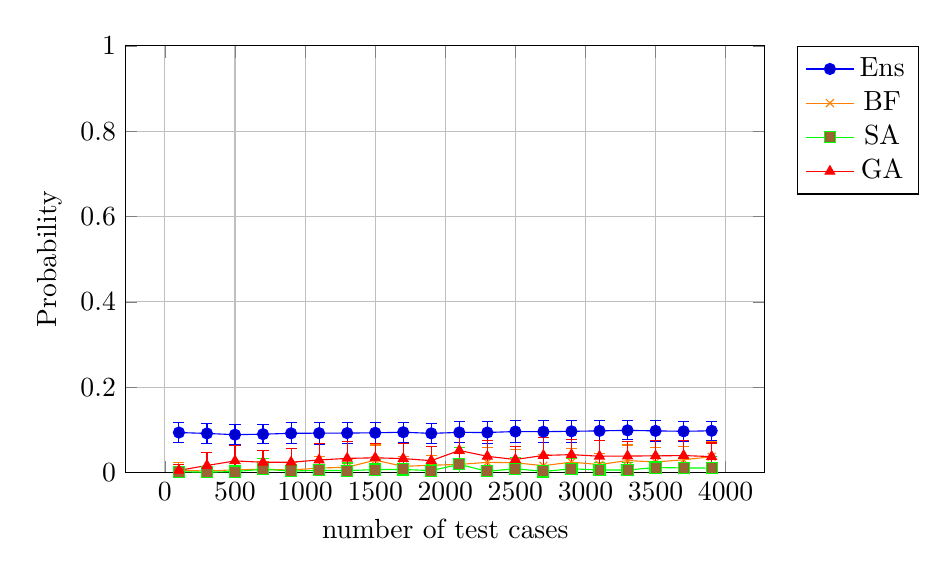
\begin{tikzpicture}
\begin{axis}[
    width=0.8\columnwidth,
    height=7cm,
    ymin=0, ymax=1,
xtick={0,500,1000,1500,2000,2500,3000,3500,4000},
xticklabels={0,500,1000,1500,2000,2500,3000,3500,4000},
    xlabel={number of test cases},
    ylabel={Probability},
    grid=major,
    legend style={at={(1.05,1)},anchor=north west},
    error bars/y dir=both,
    error bars/y explicit]
\addplot+[mark=*,color=blue,error bars/.cd,y dir=both,y explicit] coordinates {
(100, 0.09358000000000001) +- (0, 0.02435627564438588)
(300, 0.09146000000000004) +- (0, 0.02355818675673699)
(500, 0.08850000000000001) +- (0, 0.02362742267029598)
(700, 0.08976) +- (0, 0.022605363279089054)
(900, 0.09173999999999999) +- (0, 0.024392881196390565)
(1100, 0.09214) +- (0, 0.025561458551211565)
(1300, 0.09233999999999998) +- (0, 0.02439773325034743)
(1500, 0.09296000000000003) +- (0, 0.024717968346603024)
(1700, 0.0943) +- (0, 0.02332140122509883)
(1900, 0.09168000000000001) +- (0, 0.023228624143324477)
(2100, 0.09388000000000002) +- (0, 0.02459354486404079)
(2300, 0.09368000000000005) +- (0, 0.025027690786855256)
(2500, 0.09592) +- (0, 0.025309383595006504)
(2700, 0.09564000000000002) +- (0, 0.025212371436843916)
(2900, 0.09640000000000003) +- (0, 0.02607680962081058)
(3100, 0.09748000000000002) +- (0, 0.023414839181116445)
(3300, 0.09874000000000002) +- (0, 0.022271799685352856)
(3500, 0.09743999999999998) +- (0, 0.02364116092318482)
(3700, 0.09646000000000003) +- (0, 0.022818905516689133)
(3900, 0.09764000000000005) +- (0, 0.021889108278421894)
};
\addlegendentry{Ens}
\addplot+[mark=x,color=orange,error bars/.cd,y dir=both,y explicit] coordinates {
(100, 0.00578) +- (0, 0.017645361302909165)
(300, 0.0031400000000000004) +- (0, 0.011621601983077084)
(500, 0.00636) +- (0, 0.014992188442175954)
(700, 0.007460000000000001) +- (0, 0.01738895966892059)
(900, 0.00574) +- (0, 0.017159289743162328)
(1100, 0.01034) +- (0, 0.026119513387347717)
(1300, 0.012220000000000002) +- (0, 0.018983655698349287)
(1500, 0.028799999999999996) +- (0, 0.035596376793380624)
(1700, 0.014380000000000002) +- (0, 0.023847209223619898)
(1900, 0.016900000000000005) +- (0, 0.02386890214894515)
(2100, 0.018860000000000002) +- (0, 0.025503909264171683)
(2300, 0.023719999999999998) +- (0, 0.03504634832064884)
(2500, 0.022720000000000004) +- (0, 0.031759324518596914)
(2700, 0.0159) +- (0, 0.026427606159978603)
(2900, 0.024199999999999996) +- (0, 0.031016124838541652)
(3100, 0.018500000000000003) +- (0, 0.026871007059806357)
(3300, 0.027959999999999995) +- (0, 0.03651220651357292)
(3500, 0.02458) +- (0, 0.034829081210379115)
(3700, 0.029799999999999986) +- (0, 0.030755785916587137)
(3900, 0.03696) +- (0, 0.03616456716687409)
};
\addlegendentry{BF}
\addplot+[mark=square*,color=green,error bars/.cd,y dir=both,y explicit] coordinates {
(100, 0.00168) +- (0, 0.011022129873067886)
(300, 0.00066) +- (0, 0.002153402623092778)
(500, 0.00214) +- (0, 0.007122857715890184)
(700, 0.00748) +- (0, 0.025232987803060263)
(900, 0.0034599999999999995) +- (0, 0.013990098539426274)
(1100, 0.00482) +- (0, 0.013466041946848585)
(1300, 0.004320000000000001) +- (0, 0.017955091370484556)
(1500, 0.00676) +- (0, 0.022806694326939384)
(1700, 0.007040000000000002) +- (0, 0.01870278818022291)
(1900, 0.0043) +- (0, 0.015326714040044792)
(2100, 0.018959999999999998) +- (0, 0.039736355635408664)
(2300, 0.00254) +- (0, 0.00815965685553014)
(2500, 0.00884) +- (0, 0.02662081432079118)
(2700, 0.00234) +- (0, 0.0108017572266587)
(2900, 0.008579999999999999) +- (0, 0.025186723097857792)
(3100, 0.0057799999999999995) +- (0, 0.018366217879129974)
(3300, 0.005860000000000001) +- (0, 0.018002278767320724)
(3500, 0.01146) +- (0, 0.02817236306766485)
(3700, 0.01068) +- (0, 0.024448563248132993)
(3900, 0.0102) +- (0, 0.02820840806770715)
};
\addlegendentry{SA}
\addplot+[mark=triangle*,color=red,error bars/.cd,y dir=both,y explicit] coordinates {
(100, 0.004940000000000001) +- (0, 0.013418552493484837)
(300, 0.016300000000000002) +- (0, 0.030174492539229218)
(500, 0.027100000000000003) +- (0, 0.035932618346350566)
(700, 0.02388000000000001) +- (0, 0.02838269090232887)
(900, 0.023939999999999993) +- (0, 0.03247568006860469)
(1100, 0.02927999999999999) +- (0, 0.03774297610016942)
(1300, 0.032979999999999995) +- (0, 0.03935836917975383)
(1500, 0.03433999999999998) +- (0, 0.034060935790708645)
(1700, 0.03252) +- (0, 0.03604376025141141)
(1900, 0.027719999999999988) +- (0, 0.0331139282613519)
(2100, 0.05156000000000001) +- (0, 0.0383560973520721)
(2300, 0.037799999999999986) +- (0, 0.03758799200352612)
(2500, 0.030379999999999994) +- (0, 0.031042360787564248)
(2700, 0.039880000000000006) +- (0, 0.041404741915162614)
(2900, 0.04181999999999999) +- (0, 0.034813608645740485)
(3100, 0.03803999999999999) +- (0, 0.03602831086345112)
(3300, 0.03851999999999999) +- (0, 0.03317685448425435)
(3500, 0.038880000000000005) +- (0, 0.03587258631573127)
(3700, 0.039599999999999996) +- (0, 0.03597107681661669)
(3900, 0.0372) +- (0, 0.03197128813961243)
};
\addlegendentry{GA}
\end{axis}
\end{tikzpicture}
\caption{BrokenPeterson}
\label{fig:BrokenPeterson}
\end{figure}
